\chapter{Machine Learning}

\section{Building a Thinking Machine}

\subsection{Conscious Decision Making As an Algorithm}

\subsection{Fumbling Towards a Solution}

\subsection{Tools for Fumbling Faster}

\section{An Analysis Pipeline}

\section{Modelling a Brain}

\subsection{Neural Layers}

\subsection{Classification and Regression}

\section{Neural Architectures}

\subsection{Convolutional Nets}

\subsection{Generative Adversarial Nets}

\subsection{Recurrent Neural Nets}\label{sec:RNN}

%%%%%%%%%%%%%%%%%%%%%%%%%%%%%%%%%%%%%%%%%%%%%%%%%%%%%%%%%%%

Machine learning is an area of computer science in which we attempt to create intelligent systems that are able to make complex, human-level decisions. It has seen use in recent years in areas as diverse as self-driving cars, language processing, and automatic crop harvesting. In recent years, many machine learning techniques have started being applied to the realm of high-energy physics. Due to very high volumes of data production, especially for planned next-gen colliders such as the HL-LHC, and due the complexity involved in reconstructing each collision event, machine learning has been applied to applications such as track reconstruction, vertex-finding, and jet identification, and was used in the Higgs discovery. The field is extremely broad with many applications, so I will only attempt to describe a few basic ideas here.

Boiled down to its fundamentals, the goal of a machine learning process is  to take a set of input data, and to generate the optimal outputs. For instance, a facial recognition system may take as its inputs a set of pixels originating from a camera or video feed, and output a pointer to a name in a database of people. A translation program may take a string of characters in one language as text input and output another string in a different language. A drone with obstacle avoidance may take input from visual systems and from mounted sensors, and output instructions to its various motors. Even an organic entity takes chemical, physical, and internal inputs from its environment, and outputs chemical and electrical signals to its muscles and organs. There are two major classifications of machine-learning algorithms. One type is supervised, where a system is fed a series of training examples, and is told explicitly what type of output the system should be attempting to obtain for each example. This is the case for an image-classification algorithm, which may be fed many different input images, along with labels for each image. The other major type of machine learning algorithm is unsupervised. In this case, the algorithm is still fed input data, but is not told what the output should be. This is generally the case for clustering algorithms, such as those used for data compression and error/outlier detection.

To build a particle recognition system, we will eventually require unsupervised learning in order to implement systems that recognize and zoom in on energy clusters. However, in the interest of conciseness, I will focus only on supervised algorithms here. As its name suggests, the field of machine learning is generally focused on how to get an algorithm to "learn" from input data. In a supervised learning example, the algorithm takes the form of a complicated expression with many tunable parameters. This expression may be in the form of a series of matrix operations, or as a chain of cut-based classifiers, or in general any other form of an input-output system with tunable components. This algorithm begins with some initialized parameters, and is fed a chunk of input data (which may be composed of one or several input examples). The algorithm then spits out its outputs, which are compared to the correct outputs. The accuracy of the response is then quantified using a "loss function", which in practice is often either the L2 distance, the logistic loss function, or the cross entropy loss. I will now talk about two very common algorithms, the boosted decision tree (BDT) and neural net (NN).

\subsection*{BDT}

Simply speaking, a decision tree is simply a series of branching paths based on input data, which one can follow to reach a conclusion. An example of a very simple decision tree is shown in Figure~\ref{decision_tree}. Decision trees are similar to how objects and signal regions are selected in a traditional high-energy-physics analysis. For example, one may ask whether an event has more than, less than, or equal to three leptons. If the event has exactly three leptons, one may ask whether the top two leptons have dilepton mass within a certain range, etc. Based on these decisions, an experimenter can decide what signal region an event belongs in. As another example, imagine that we are trying to determine what kind of particle we have seen in an event. We could ask whether the particle left a track in the inner detector, whether the amount of energy it deposited in the calorimeter is in a certain range, etc. Given a random ordered set of input variables, an optimal decision tree can be calculated for decisions made in that specific order.

A boosted decision tree is created by combining many different decision trees together \cite{BDT}. Any given decision tree can be very weak, containing only a small number of branches and a small maximum depth. However, by taking the weighted results of many decision trees together, we can get a more accurate result than can be achieved by any single tree. For the sake of space, the AdaBoost BDT training algorithm will not be discussed here.

\begin{figure}[t]
    \centering
    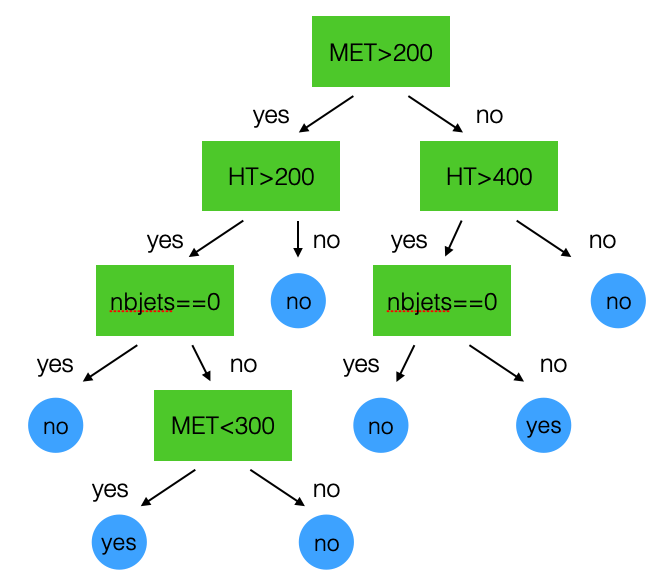
\includegraphics[width=0.5\linewidth]{images/decision_tree.png}
    \caption{An example of a decision tree that a child may use to classify a household pet.}
    \label{decision_tree}
\end{figure}

\subsection*{Neural Net}

A neural net is a machine learning architecture based on the physical structure of neurons in the human brain \cite{neural_net}. The basic unit of a neural net is a neuron, which has a numerical value, one or more inputs, and one or more outputs. These neurons are connected together so that the output of one neuron becomes the input of one or more other neurons. Here we will only consider simple feed-forward neural nets, where all the inputs to a neuron come from neurons closer to the beginning of the net, and all the outputs of that neuron go to neurons nearer the end of the net. That is, there are no "loops", and there are no connections between neurons at the same depth. The input values for an event form the first layer of neurons, and the output is derived from the last layer. Each link between neurons is associated with a "weight", or multiplicative constant. Each neuron is also associated with a "bias", or an additive constant. Letting $y_i$ be the value of the $i^{th}$ neuron, $w_{i,j}$ be the value of the weight between neurons $i$ and $j$, and $b_i$ be the bias associated with neuron $i$, we see that the value of a neuron is equal to $y_j = \sum{w_{i,j}y_i} + b_j$. Each neuron is also typically followed by a nonlinear "activation" function, so that the result of the entire net is not simply equivalent to a single matrix operation on the input. We see then that for a given set of weights and biases, we can calculate the output value for a net given any inputs.

In order to train a neural net, we use "back-propagation", meaning that for each event (or set of events) we perform gradient descent on each weight and bias in order to minimize the resulting loss function. Over the course of many events, the net can fall into a state where it produces the correct outputs with high accuracy. In this way, the neural net training is simply a form of function optimization. Many important topics, such as how to weight initialization, methods of gradient descent, net architectures, etc. will not be discussed in this paper.

\begin{figure}[t]
    \centering
    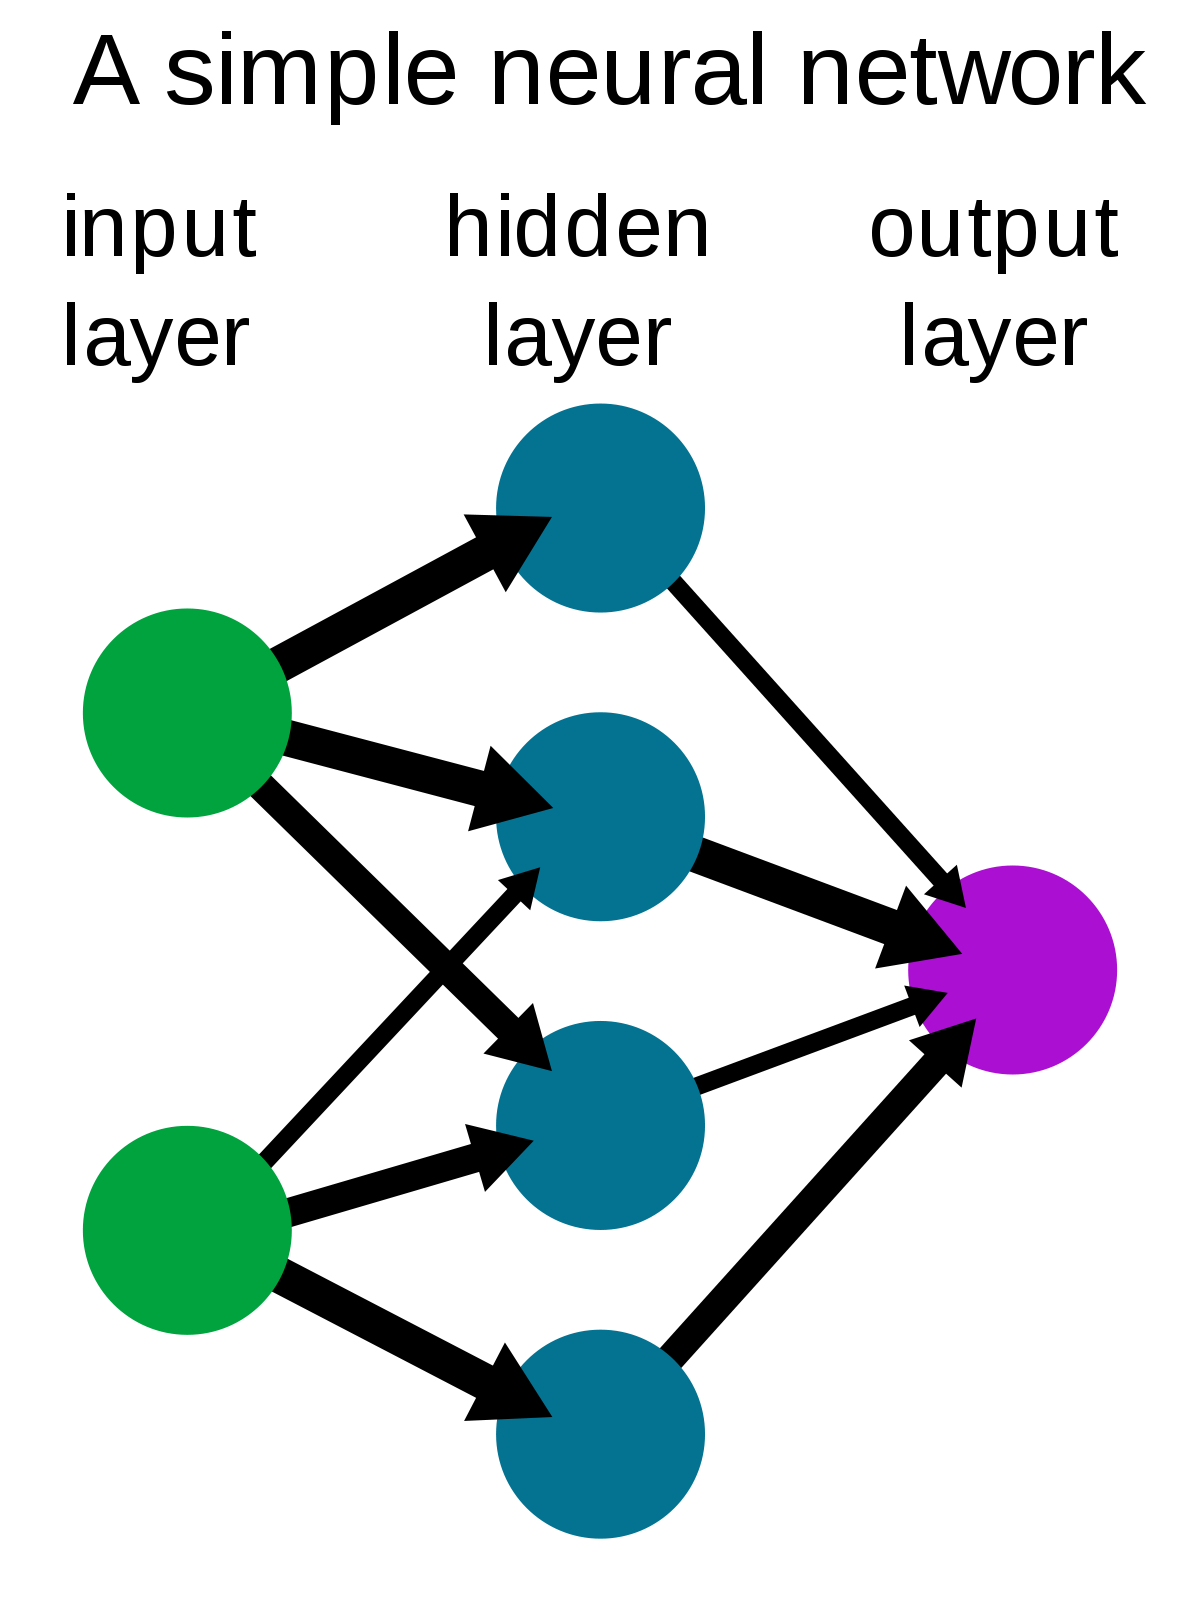
\includegraphics[width=0.5\linewidth]{images/neural_net.png}
    \caption{A diagram showing a typical densely-connected neural net.}
    \label{neural_net}
\end{figure}